\documentclass[11pt]{article}
\usepackage{placeins} 
\usepackage[labelsep=period]{caption}
\usepackage[utf8]{inputenc}
\usepackage[T1]{fontenc}
\usepackage{graphicx}
\usepackage{subcaption}
\usepackage{grffile}
\usepackage{longtable}
\usepackage{wrapfig}
\usepackage{rotating}
\usepackage[normalem]{ulem}
\usepackage{amsmath}
\usepackage{textcomp}
\usepackage{amssymb}
\usepackage{capt-of}
\usepackage[hidelinks]{hyperref}

\usepackage{float}
\usepackage{array}
\usepackage{soul}
\usepackage{tabularx}
\usepackage[english]{babel}
\usepackage{lineno}

\usepackage{xcolor}
\usepackage[backend=biber, sorting=none]{biblatex}

\newcommand{\R}[1]{\label{#1}\linelabel{#1}}
\newcommand{\lr}[1]{~\lineref{#1}}

\usepackage{url}
%\urlstyle{same}
% Make URLS show better
%\Urlmuskip=0mu plus 1mu\relax

\topmargin 0mm \oddsidemargin 2mm \evensidemargin 2mm \textwidth 160mm \textheight 578.201 pt

\addbibresource{report_cdc_forecasting_covid19_NotreDame-FRED.bib}

\date{}
\title{Forecasting COVID-19 mortality in the US Midwest}
\author{Guido Espa\~na,  Rachel Oidtman\textsuperscript{*}, Sean Cavany\textsuperscript{*}, Alan Costello, \\Annaliese Wieler, Anita Lerch, Carly Barbera,  Marya Poterek, Quan Tran,\\ Sean Moore, and T. Alex Perkins\\
  \textsuperscript{1}University of Notre Dame, United States\\  
  \textsuperscript{*} Equal contribution
}
\begin{document}  
\linenumbers
\maketitle

\setcounter{page}{1}
\begin{abstract}
We used an existing agent-based model, FRED (Framework for Reconstructing Epidemic Dynamics), which was originally developed by the University of Pittsburgh in response to the 2009 influenza pandemic. We adapted FRED for modeling COVID-19 in the US by updating epidemiological parameters based on studies to date. FRED explicitly models transmission dynamics of a pathogen in a realistic population, and it allows for the impacts of NPIs to be modeled explicitly (e.g., school closure results in agents representing children staying home). Our aim was to leverage the realism and geographic and demographic appropriateness of this model for the US to make short term forecasts of COVID-19, with a focus on incidence of cases and deaths and the impacts of NPIs thereon. At this time, we limit our analysis to seven Midwest states comprising a coalition of states coordinating their response: Illinois, Indiana, Kentucky, Michigan, Minnesota, Ohio, and Wisconsin.
\end{abstract}

\section{Methods}
\subsection{Model description}

We used an existing agent-based model, FRED (Framework for Reconstructing Epidemic Dynamics) which was developed by the university of Pittsburgh in response to the 2009 influenza pandemic \cite{grefenstette2013}. We modified the model parameters to represent the natural history of COVID-19 and calibrated a set of parameters to reproduce current trends of deaths due to COVID-19 in the US. FRED simulates the spread of the virus in a population by recreating interactions among people on a daily basis. To accurately represent the population of each of the states simulated, we used a synthetic population of the US that represents demographic and geographic characteristics of the population in 2010 \cite{Wheaton2012}. Each human is modeled as an agent that visits a set of places defined by their activity space. This activity space contains places such as households, schools, workplaces, or neighborhood locations. Transmission of SARS-CoV-2 can occur when an infected person visits the same location as a susceptible person on the same day. Numbers of contacts per person are specific to each place type. For instance, school contacts do not depend on the size of the school but the age of the agent. In previous studies using FRED, these contact rates have been  adjusted to represent the observed attack rates of influenza \cite{grefenstette2013, Mossong2008_PLOS_Medicine}. Given the uncertainty on the attack rates for each place type for SARS-CoV-2, we used the same calibrated contact patterns and adjusted the transmission parameters for SARS-CoV-2. This means that although our model conserves the same contact patterns than for flu, the attack rate for each type of place is different. Estimates on the attack rate for different places would inform better the model.

In the model, infected agents have a probability to stay at home if they develop symptoms. Those who do not stay at home continue their daily activities. Public health interventions are included in the model to represent the changes in agents’ behavior in response to an epidemic. We limited this interventions to school closure and shelter in place. Schools are closed on a specific date to represent state-level guidelines \cite{ihme_covid19_forecasting}. In the case that schools are closed, students limit their activity space to household or neighborhood locations. Shelter-in-place interventions reduce each agent’s activity space to their household at a compliance level from 0-100\%, which was estimated as part of the model calibration. Agents who do not comply with the shelter-in-place orders continue with their daily routines. We used state-level orders to determine the date at which people are advised to shelter in place \cite{ihme_covid19_forecasting}. 

\subsection{Model parameters}
For the infectious period, we referred to estimates by He et al. that 44\% of transmission occurs before symptom onset and that infectiousness peaks 0.6 days before the onset of symptoms, implying that infectiousness is gamma distributed with shape and rate parameters 2.47 and 0.775\cite{He2020_Nature}. In FRED, infectiousness is uniformly distributed through an individual’s infectious period. To accomodate He et al.’s findings about the distribution of infectiousness, we chose a gamma distributed infectious period so that the 44th and 97.5th percentiles of average infectiousness (accounting for differing lengths of the infectious periods) matched that of the infectiousness distribution found by He et al. These two constraints ensured a realistic amount of presymptomatic transmission, and that individuals were not infectious for an unrealistic length of time. We estimated the infectious period parameters using the optim function in R, finding that the shape and rate parameters of the infectious period distribution were 9.01 and 1.42 respectively, implying a mean infectious period of 6.35 days. Finally, we truncated the distribution at the 99.9th percentile. As a result, we obtained an infectious period with a median of 7 days (IQR: 6-9) in our simulations (Figure \ref{fig_params_periods}, top-left panel). 

We used a lognormal distribution for the incubation and symptomatic periods with medians 5.06 days and 20.8 days respectively \cite{Lauer2020_Annals,Bi2020_LancetID}, both truncated at the 99.9th percentile. We used a gamma distribution for the time to death with mean 17.8 days, as estimated by Verity et al. \cite{Verity2020_LancetID}. This was truncated at the maximum duration of symptoms observed from patient records. In FRED, case fatality risk is determined by a daily probability of death, conditional on experiencing symptoms. Hence, the age-specific CFR is determined by the distribution of the daily probability of death and the symptomatic period distribution. The resulting CFR closely matched the age-stratified CFR used to generate the daily probabilities (Figure \ref{fig_age_cfr}) \cite{Wu2020_Nature}.

We estimated the age-adjusted probability of being symptomatic from the age distribution of cases in China \cite{ChinaCDC2020_weekly}. We did this by assuming that exposure did not vary by age, that 50\% of infections were symptomatic overall, and that the difference in the number of infections was entirely due to different probabilities of symptoms by age and the age distribution of individuals in China (“Population Pyramids of the World from 1950 to 2100” 2019). This gave a steep increase in the probability of symptoms by age, with the highest probability in the 70-79 age group and the lowest in the 0-9 age group (Figure \ref{fig_age_symp}). The resulting symptomatic period distribution among agents in a simulation is presented in the top-right panel of Figure \ref{fig_params_periods}. Asymptomatic individuals were assumed to be 0.61 times as infectious as symptomatic individuals \cite{Perkins2020_MedRxiv}, and their latent and infectious periods have the same distribution as symptomatic individuals.

Cases that are identified may be isolated at home, following a delay of one day from symptom onset. A fraction $\rho_D$ of cases are isolated and isolation occurs following a period $t_I$. We assume that $\rho_D=0.15$, and $\bar{t_I}=2.9$ days \cite{Liu2020_NEJM,Perkins2020_MedRxiv,Russell2020_CMMID}. This implies a daily probability of detection of $p_I= \frac{\rho_D}{t_I}=0.0518$. Both serial and generation intervals have a median of 5 days (IQR: 3-7 days) in our model (Figure S2, bottom row), in line with an estimate of a median of 5.2 days for that distribution \cite{He2020_Nature}. Neither serial nor generation intervals are directly parameterized in FRED, but emerge as a combination of the infectious and incubation period distributions. Around 0.2\% of serial intervals are negative in our model (Figure \ref{fig_params_periods}, bottom-left panel), due to a combination pre-symptomatic transmission and a short secondary serial interval.

\subsection{Importations}
We separately simulated domestic and international importations following the approach of Perkins et al. \cite{Perkins2020_MedRxiv}. First, we obtained data on the number of domestically and internationally imported cases and deaths up to March 18 from line-list data compiled by the MIDAS Network (“Midas-Network/COVID-19” n.d.). We then estimated the total number of domestic and international imports based on the probability of detecting a symptomatic infection, the proportion of infections that are asymptomatic, and the case fatality risk (CFR). The CFR and asymptomatic proportion were chosen from beta distributions with means 2.3\% and 17.9\%, respectively \cite{ChinaCDC2020_weekly,Mizumoto2020_Eurosurveillance}. The probability of detecting an imported case was taken from the posterior distribution of $\rho_{travel}$ in Perkins et al., which has a median of 0.39 \cite{Perkins2020_MedRxiv}. We temporally redistribute the international imported infections according to total international incidence up to February 3, and total incidence excluding China thereafter. We temporarily distribute domestic imported infections according to total US incidence. These two importation patterns are then summed to generate a single importation pattern. This process is repeated 1,000 times and then averaged across the replicates, in order to accurately account for possible early importations, which have low probability but are epidemiologically important. Finally, the magnitude of the resulting importation curve is scaled up or down by a single calibrated parameter; this process is described in the next section.

\subsection{Model calibration}
%% UPDATE DATE!!!
We calibrated model parameters to recreate the daily number of deaths at the state level through April 29. We chose to calibrate the model to the reported number of deaths instead of the reported number of cases, as reported cases depend on the proportion of symptomatic infections, the level of reporting, the number of tests, and the accuracy of the tests. We assumed that all deaths are reported.

We calibrated four parameters: transmission probability, magnitude of importations, compliance of shelter-in-place orders, and the relative transmissibility of asymptomatic infections. We specified that transmission probability could vary from 0.3 - 1.5, magnitude of importations could vary from 0.1 - 1.5, and compliance of shelter-in-place orders could vary from 0.3 - 0.9. For the compliance of shelter-in-place orders, we assumed a linear increase in the number of people adhering to the shelter-in-place orders until the proportion of households adhering to shelter-in-place orders reached the estimated level of compliance with shelter-in-place orders (Figure \ref{fig_calibrated_parameters}). This increase was informed by mobility data reported by Google community reports, created in response to the pandemic (\url{https://www.google.com/covid19/mobility/)}. For the relative transmissibility of asymptomatic infections, we assumed a prior distribution based on estimates from Luo et al. \cite{Luo2020_Contact_MedRxiv}. We assumed that this value is distributed following a beta-binomial with a mean of 0.29.

We simulated 500 combinations of these three parameters with five replicates for each set of values using the sobol function in pomp. For each state, we then calculated the probability of the reported deaths given each parameter combination for assuming that deaths follow a Poisson distribution. 

Our model output for daily deaths and cumulative number of deaths through the calibration period closely matched the data to which it was fitted (Figures \ref{fig_deaths_cumulative}, \ref{fig_deaths_forecast}). Additionally, our model was able to accurately reproduce daily deaths outside of the timeframe to which we calibrated the model (Figure \ref{fig_deaths_forecast}). We also show estimates of the reproduction number in each of these states in figure \ref{fig_reproduction_number}. 

\begin{figure}[hb!]
\centering
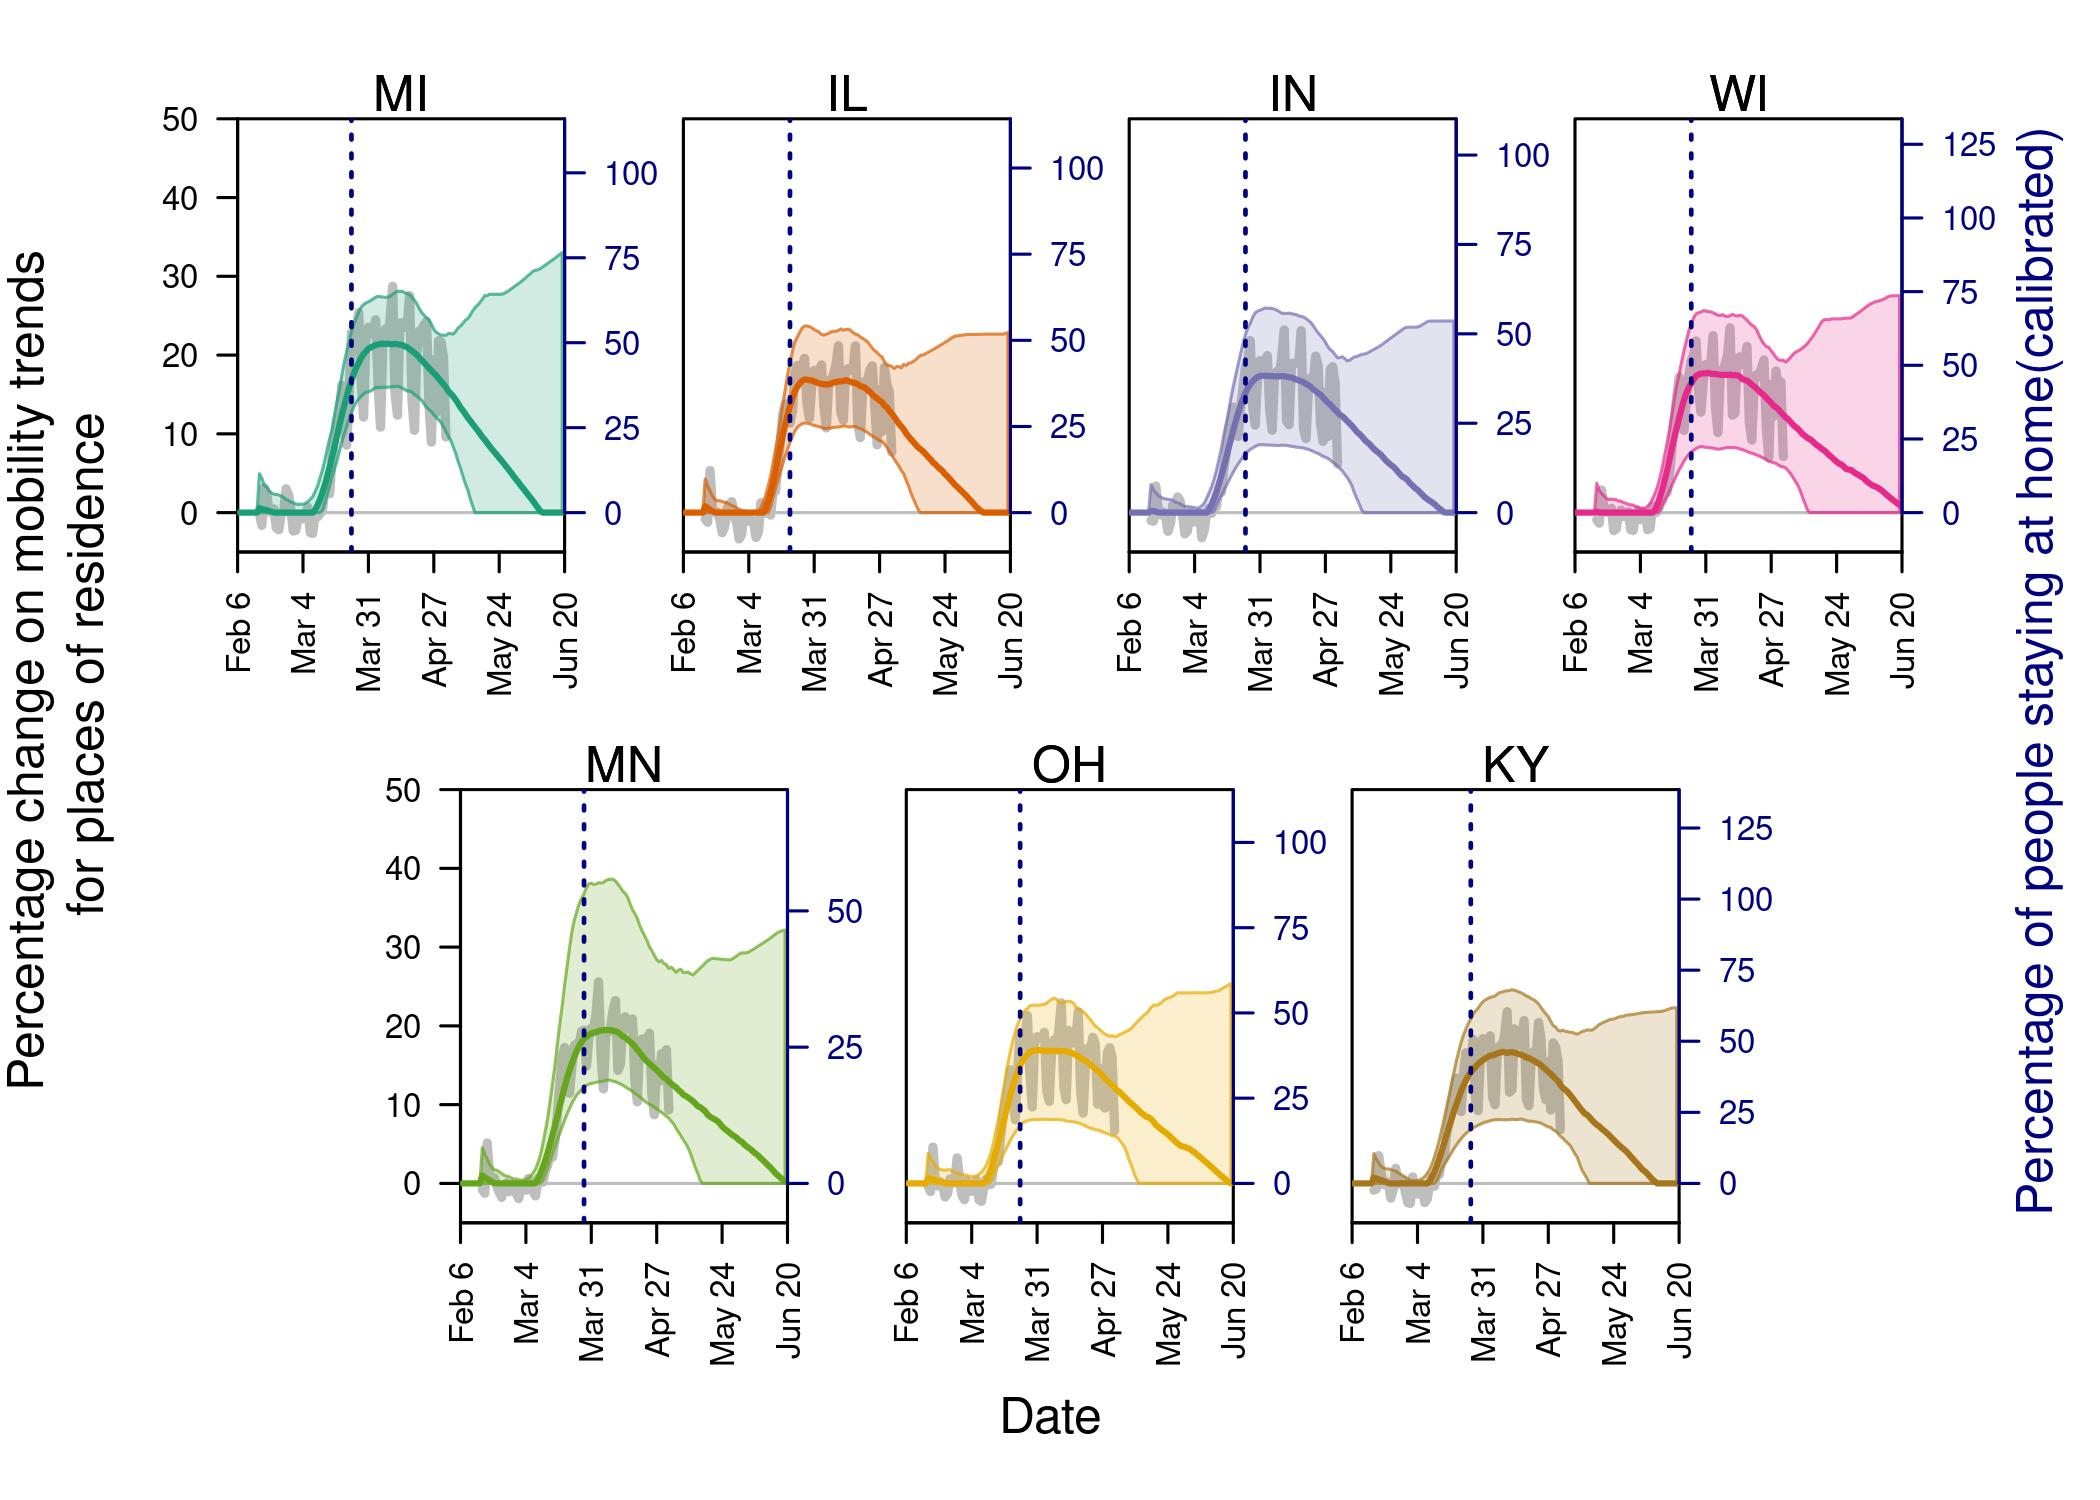
\includegraphics[width=\textwidth]{../figures/report_figure_shelter_patterns.jpeg} 
\caption{\label{fig_google_shelter} Changes in mobility patterns. Black line shows the fitted pattern in mobility to residential locations. Adherence to shelter-in-place then follows the same trend, but with the final magnitude in adherence calibrated by state to data on deaths. Colored lines represent the change in baseline mobility patterns according to the mobility reports from google.}
\end{figure}


%% AUTOMATICALLY UPDATE THE FOLLOWING PARAGRAPHS!!!!
Across states, the estimated parameters, such as the level of compliance with state orders of shelter in place, varied from state to state (Figure \ref{fig_calibrated_parameters}). These parameters were adjusted for each state to represent the state-by-state differences. The fitted values were similar across the states, except for Minnesota, which had the lowest level of compliance. The effective transmissibility parameter also varied across states, with the highest value adjusted for Minnesota to adjust for the increasing trend observed in the data. This increasing trend in Minnesota is also represented in the model with a reproduction number above 1, even after shelter-in-place orders were in place \ref{fig_reproduction_number}. Similarly, the google mobility trends show a reduction in the percentage of time spent at home in Minnesota, suggesting a reduction in the adherence to shelter-in-place orders. In the future, we will use time-varying data of people mobility patterns to account for these changing patterns. 

Our model captured the overall dynamics of the daily number of deaths reported for each of the six states considered up to the calibration period (Figure \ref{fig_deaths_forecast},\ref{fig_deaths_cumulative}). Even though we did not fit the model with data reported after the calibration period, the 95\% posterior predictive interval of our model also captured the daily number of deaths reported in the week after the prediction dataset in all six states.


\begin{figure}[hb!]
\centering
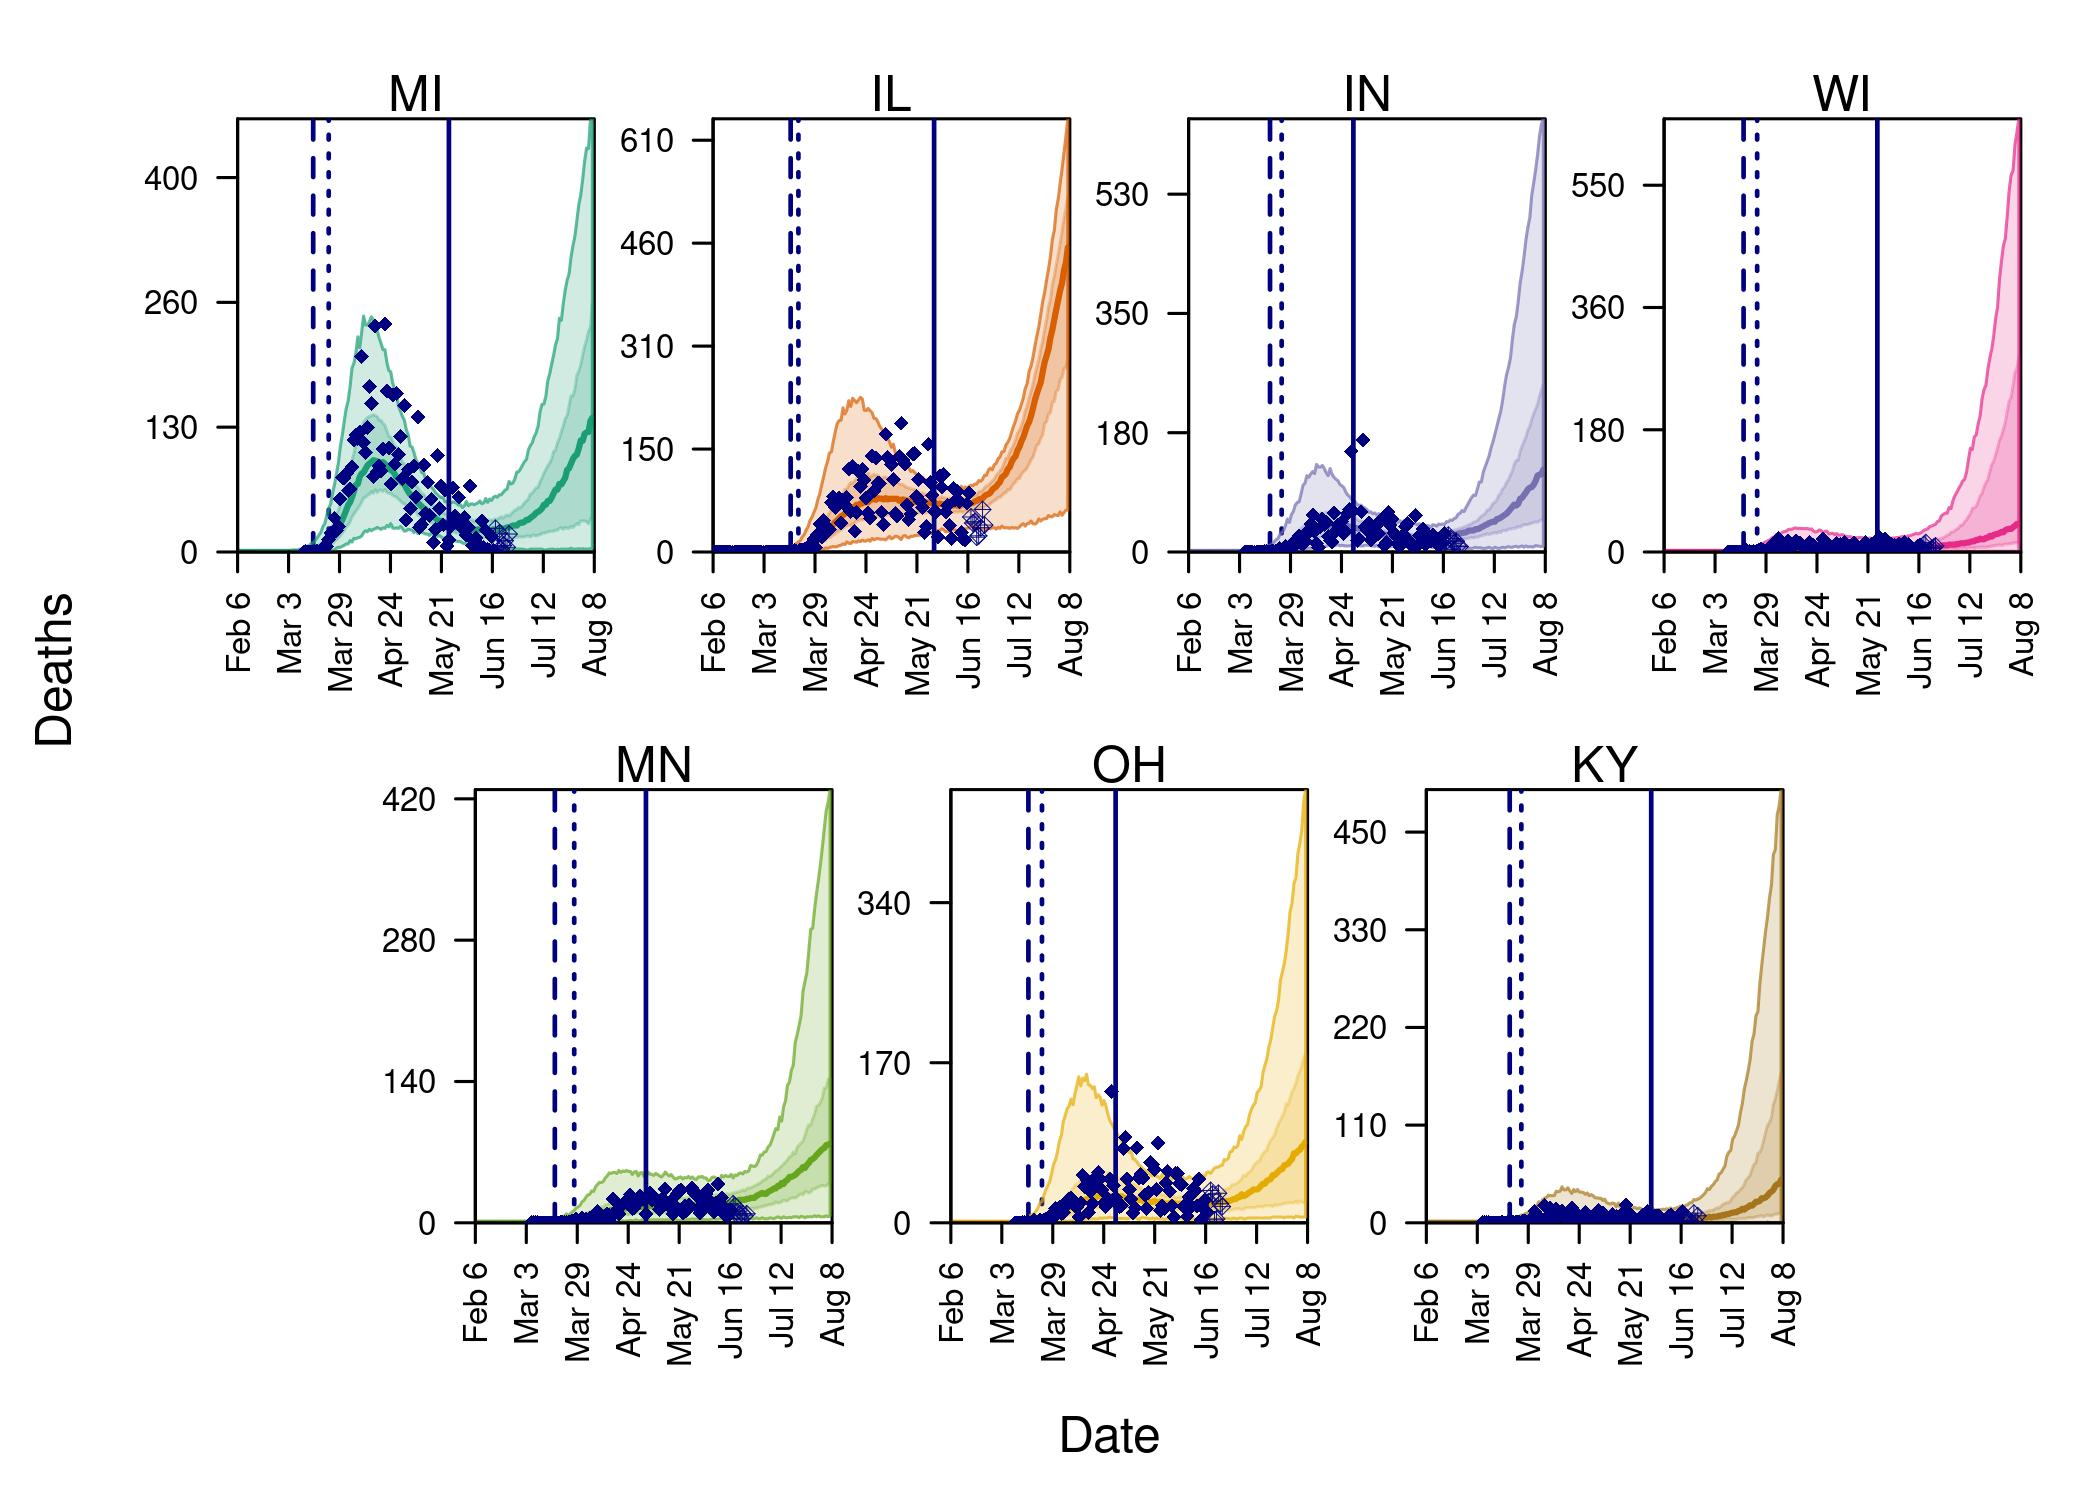
\includegraphics[width=\textwidth]{../figures/report_figure_deaths_forecast.jpeg} 
\caption{\label{fig_deaths_forecast} Projected daily deaths under two assumptions of shelter in place. The colored lines represent a scenario where shelter-in-place compliance is maintained until the end of the simulation. Black diamonds show the data used to fit the model, while empty diamonds show the recent data not used in the fitting process. Navy dashed line shows the time of schools closure and the dotted navy line shows the time of shelter-in-place orders.}
\end{figure}

\begin{figure}[hb!]
\centering
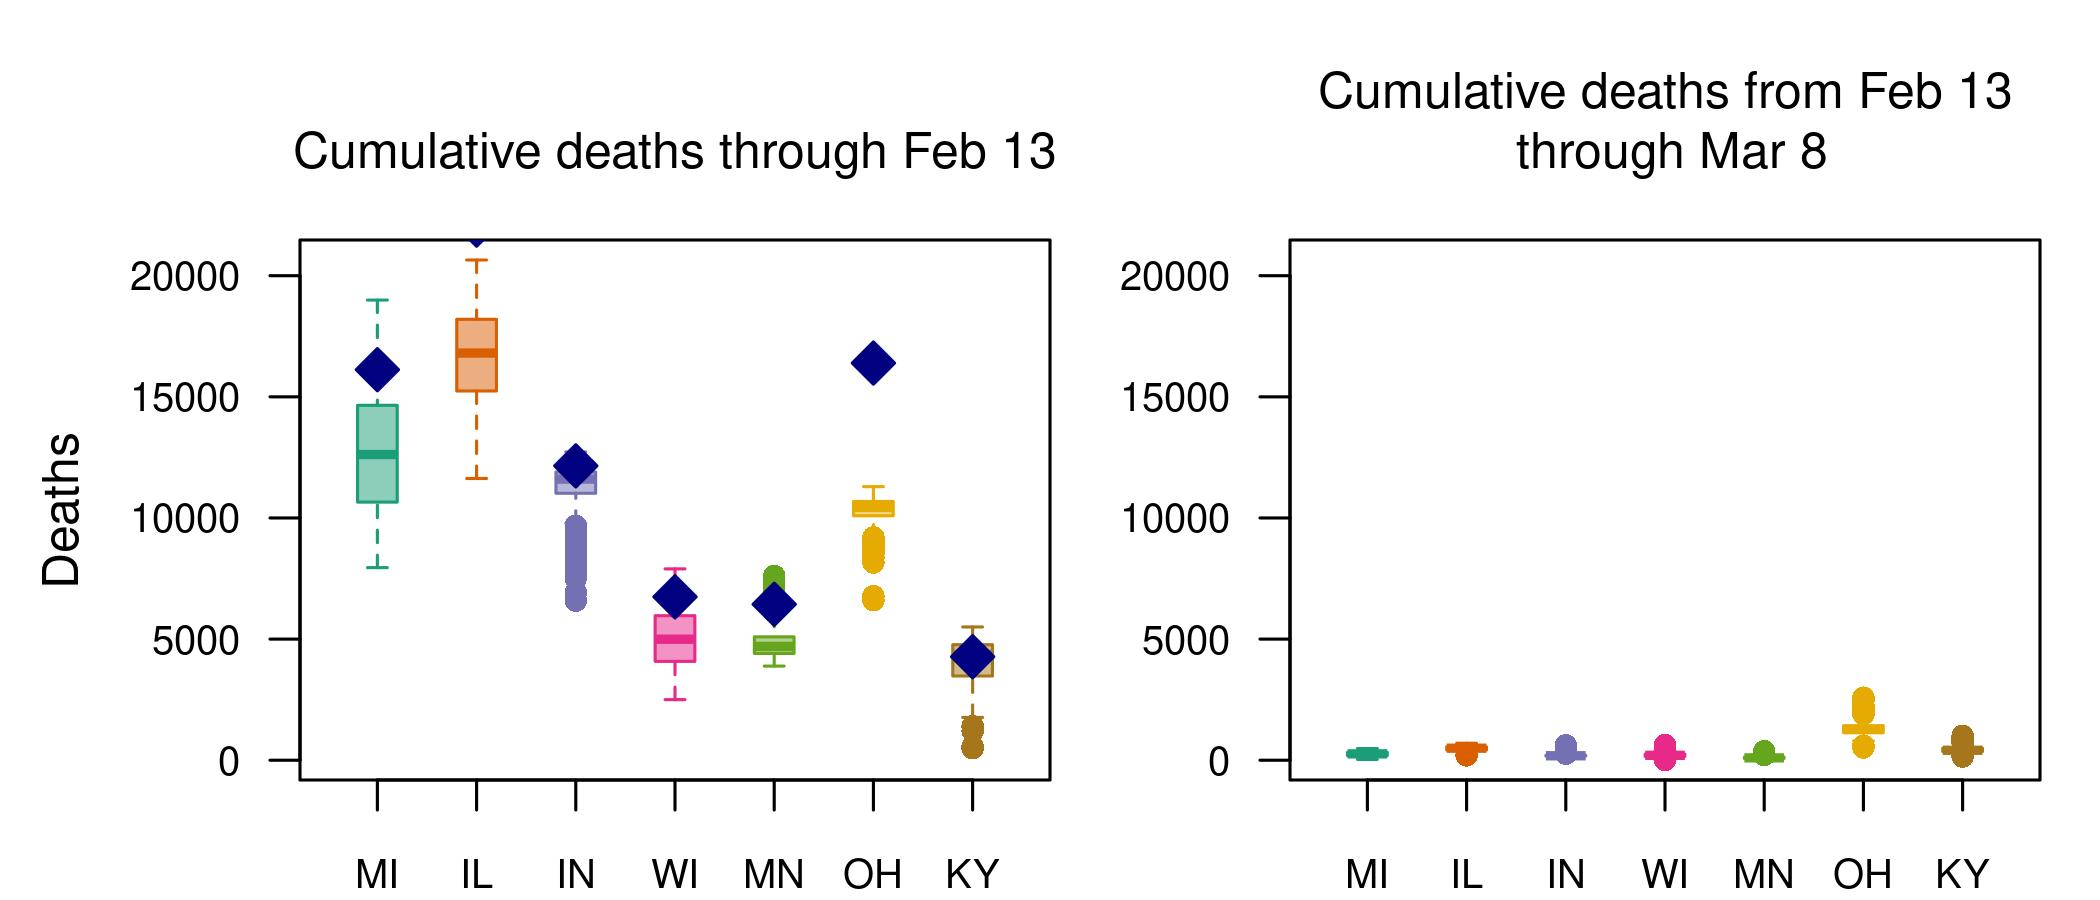
\includegraphics[width=\textwidth]{../figures/report_figure_deaths_cumulative.jpeg} 
\caption{\label{fig_deaths_cumulative}Estimated and projected cumulative deaths in the calibration period(left column) and June 15 (right column). Left panel: Navy diamonds denote empirical data.}
\end{figure}


\begin{figure}[hb!]
\centering
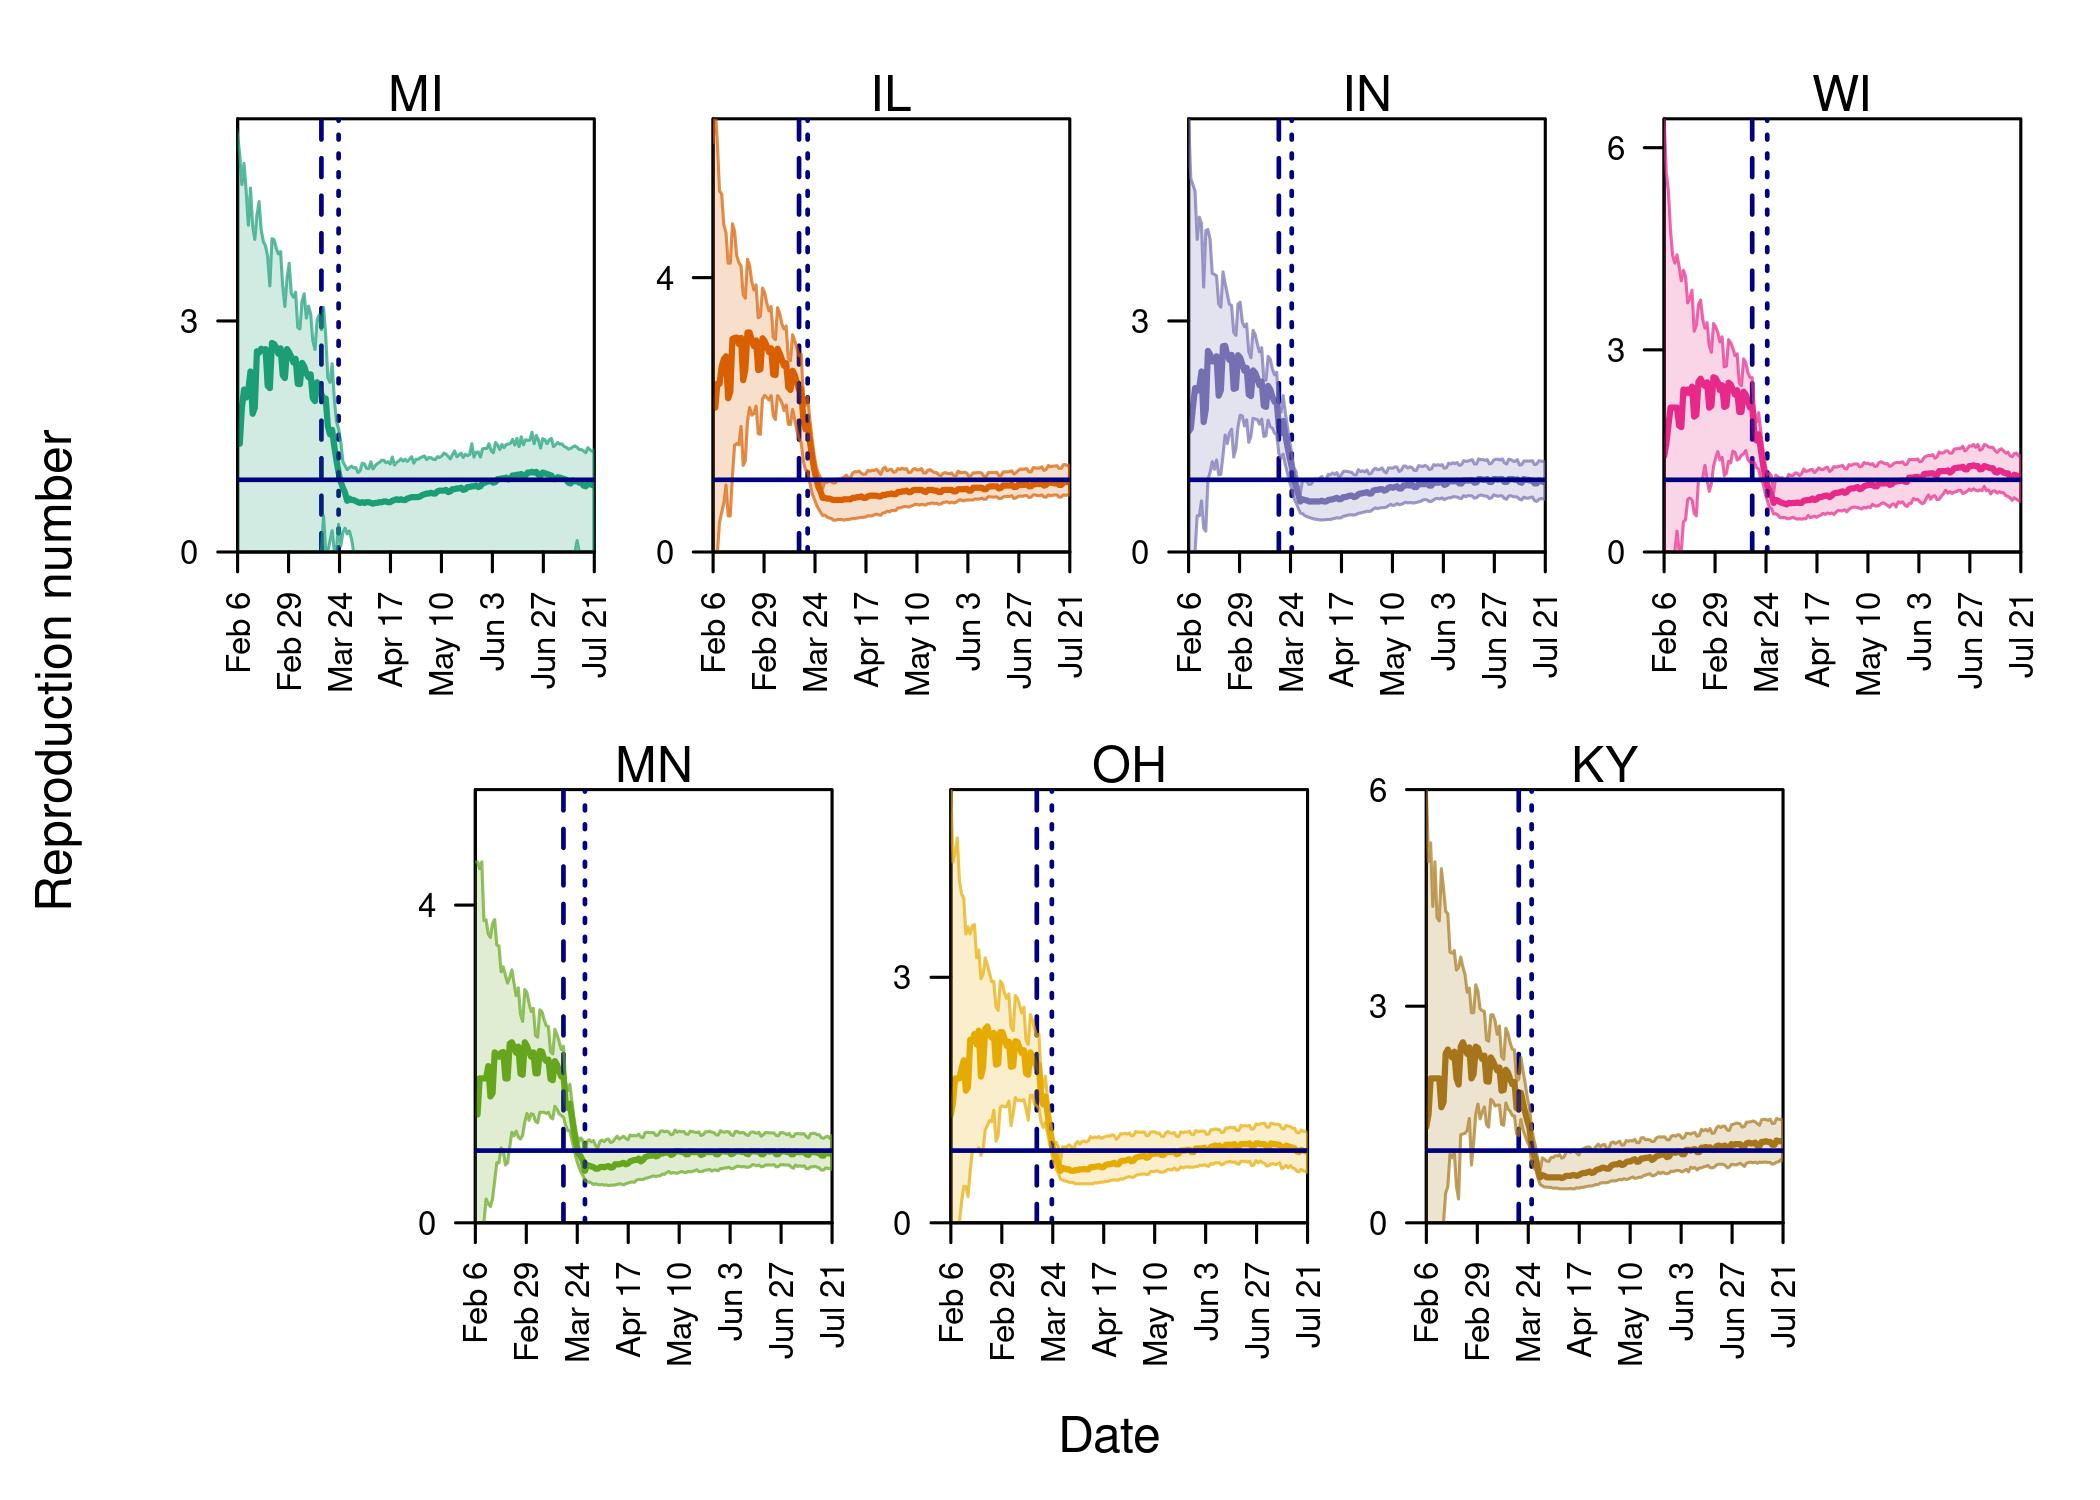
\includegraphics[width=\textwidth]{../figures/report_figure_reproduction_number.jpeg} 
\caption{\label{fig_reproduction_number} Estimated and projected reproduction number for six states in the Midwest. Gray bands show a scenario where stay-at-home orders remain. Color bands show a scenario where stay-at-home orders are lifted at a specific date denoted by the solid navy line.}
\end{figure}




\subsection{Model limitations}

A strength of our study is that we calibrate our model to data on deaths from each state. Data on deaths is more robust to variability in reporting rates than the number of cases, and calibrating our model to them helps ensure our model is accurately reproducing transmission dynamics in these states. Nonetheless, deaths can also be underreported, and if this is the case it may be that we underestimated transmission slightly in our model. Furthermore, reported deaths have a larger delay than the number of daily cases, which reduces our ability to capture recent changes in the transmission dynamics. Our model calibration could be improved further by careful incorporation of data on reported cases and test results by state. Another limitation of our current model calibration is that we assumed a fixed proportion of adherence to shelter-in-place orders. Surveys in Italy suggest that this proportion decreases if  shelter-in-place orders are extended \cite{Briscese2020_NBER}. Qualitatively, our forecasts on the number of daily reported deaths are in agreement with most of the states in this study. Importantly, the model is unable to capture the recent increase in deaths in several states. This could be due in part to large recent outbreaks in enclosed facilities, such as a prison in Ohio, and a recent upturn in the number of deaths in Minnesota. 

Currently, our model projects a greater effect of school closures than stay-at-home orders on transmission. This is not in line with other studies’ findings. There are two likely reasons for this. One is that our model, designed for flu initially, overweights transmission in schools and does not adequately represent other transmission locations. The second is that we may underestimate the compliance with shelter-in-place. We expect to resolve these issues in future model iterations. A final limitation of our model is that we don’t account for the full range of uncertainty in our model parameters. Though we account for stochasticity in the transmission process, we use single estimates for the moments of the underlying distributions. To overcome this issue, we estimate the relative transmissibility of asymptomatic infections with an informed prior distribution based on literature estimates. 

%% FUNDING STATEMENT SOMEWHERE
\clearpage
\printbibliography


\section*{Supplementary material}
\setcounter{table}{0}
\renewcommand{\thetable}{S\arabic{table}}%
\setcounter{figure}{0}
\renewcommand{\thefigure}{S\arabic{figure}}%

\begin{figure}[hb!]
\centering
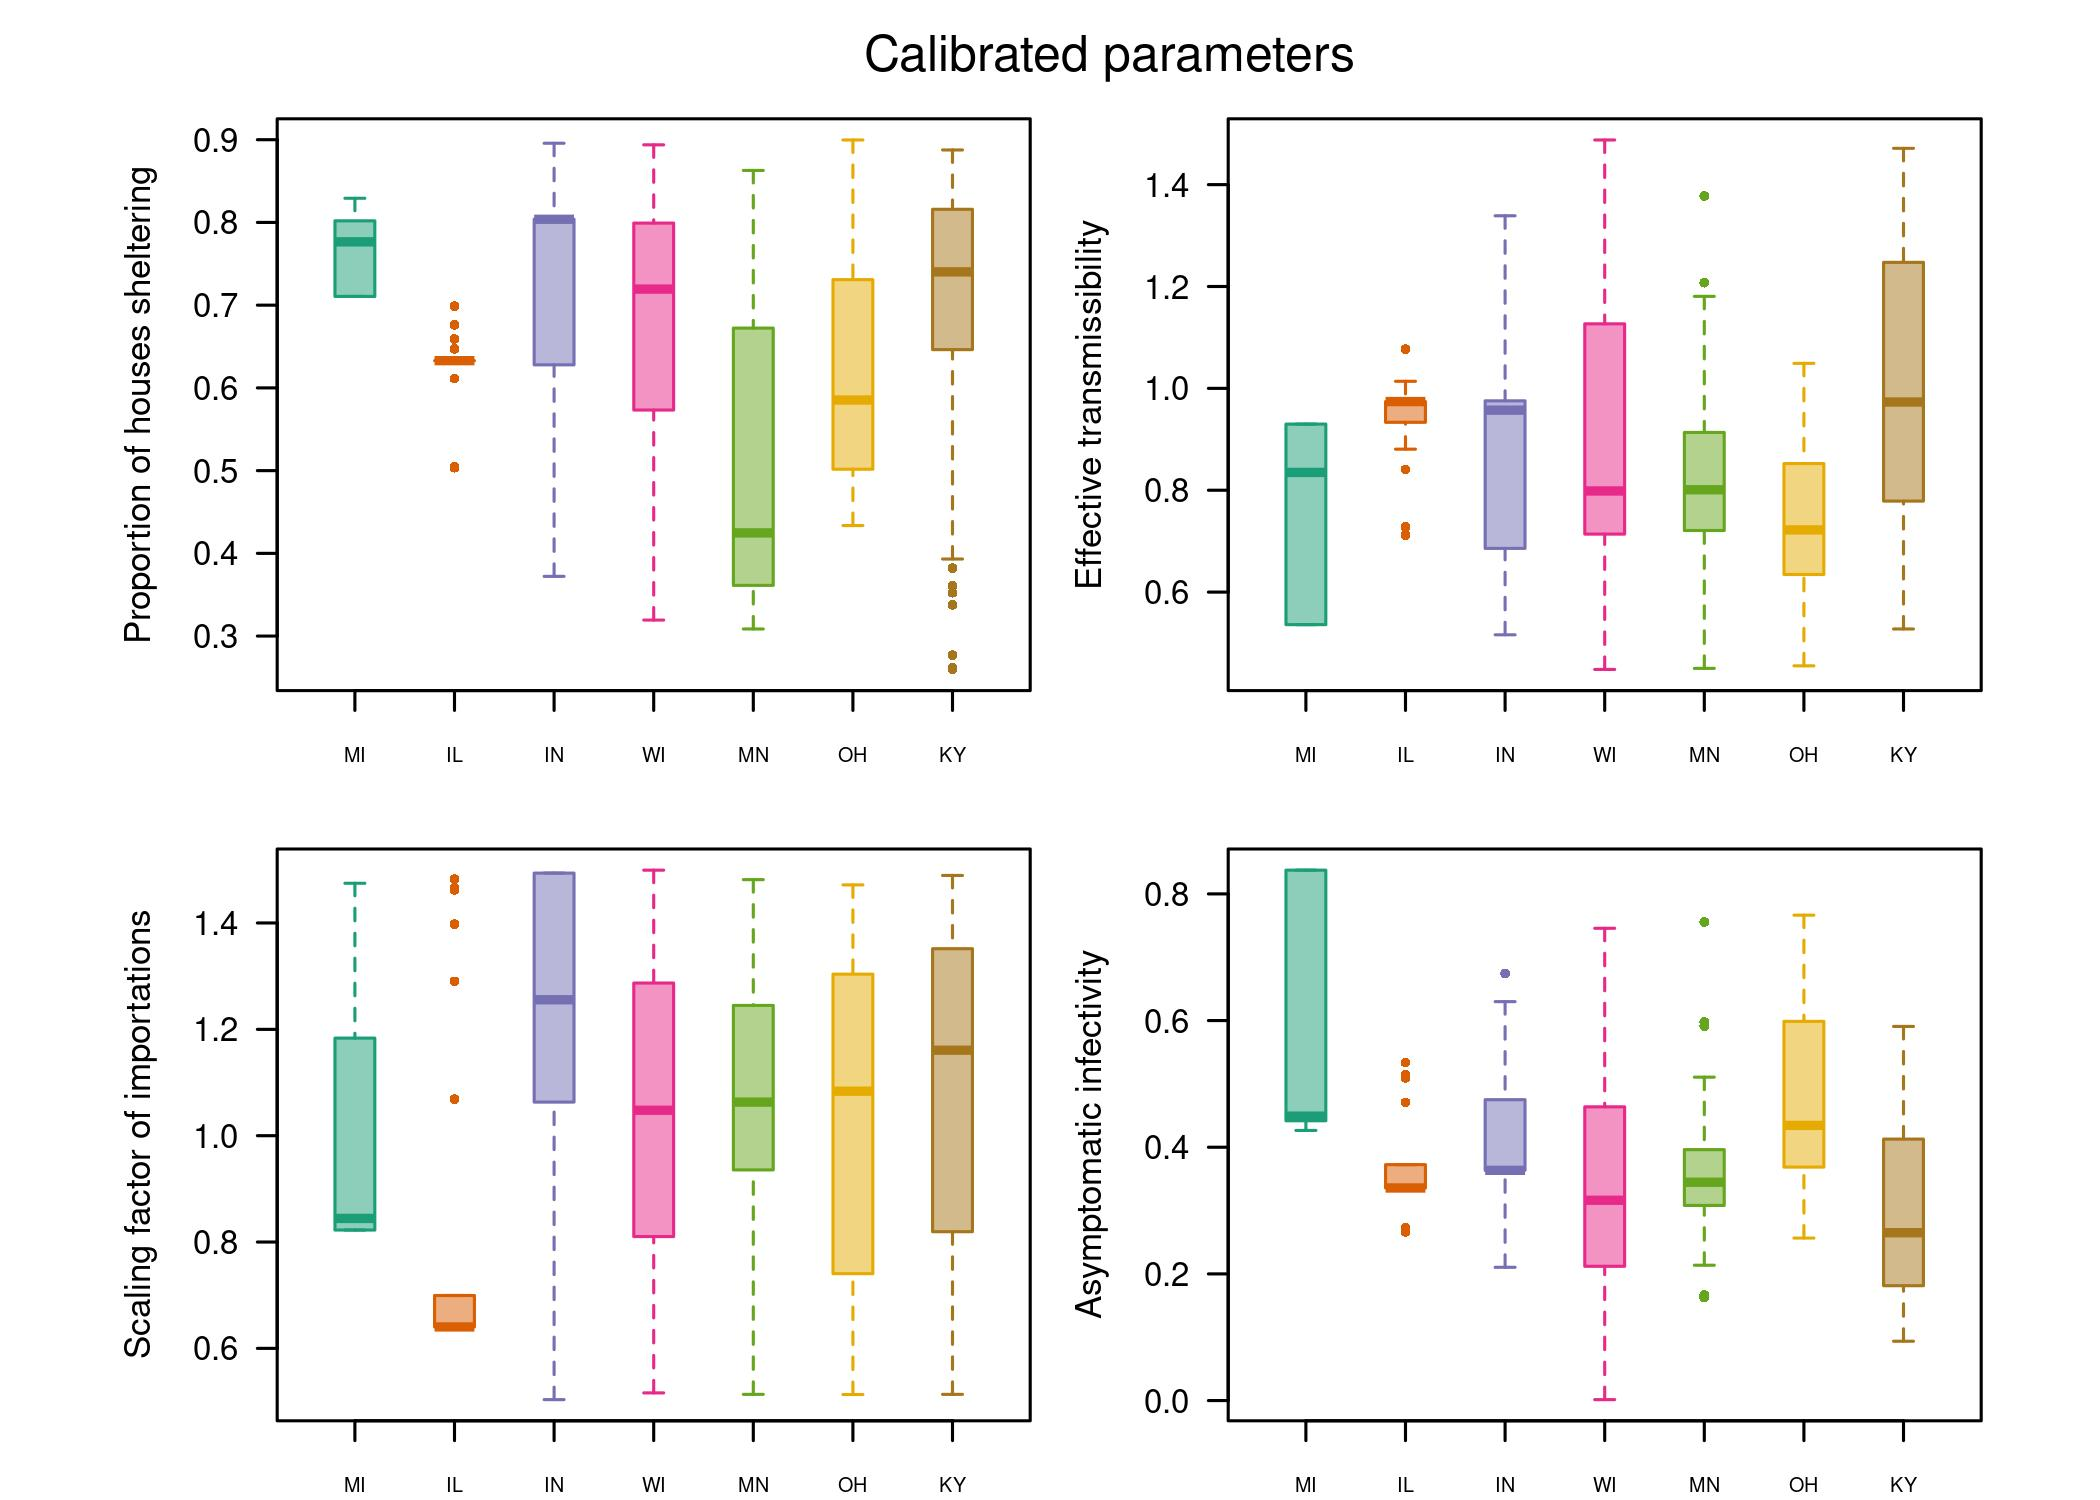
\includegraphics[width=\textwidth]{../figures/report_figure_calibrated_parameters.jpeg} 
\caption{\label{fig_calibrated_parameters}Distribution of calibrated parameters. Calibrated parameters based on 500 different parameter combinations.}
\end{figure}

\begin{figure}[hb!]
\centering
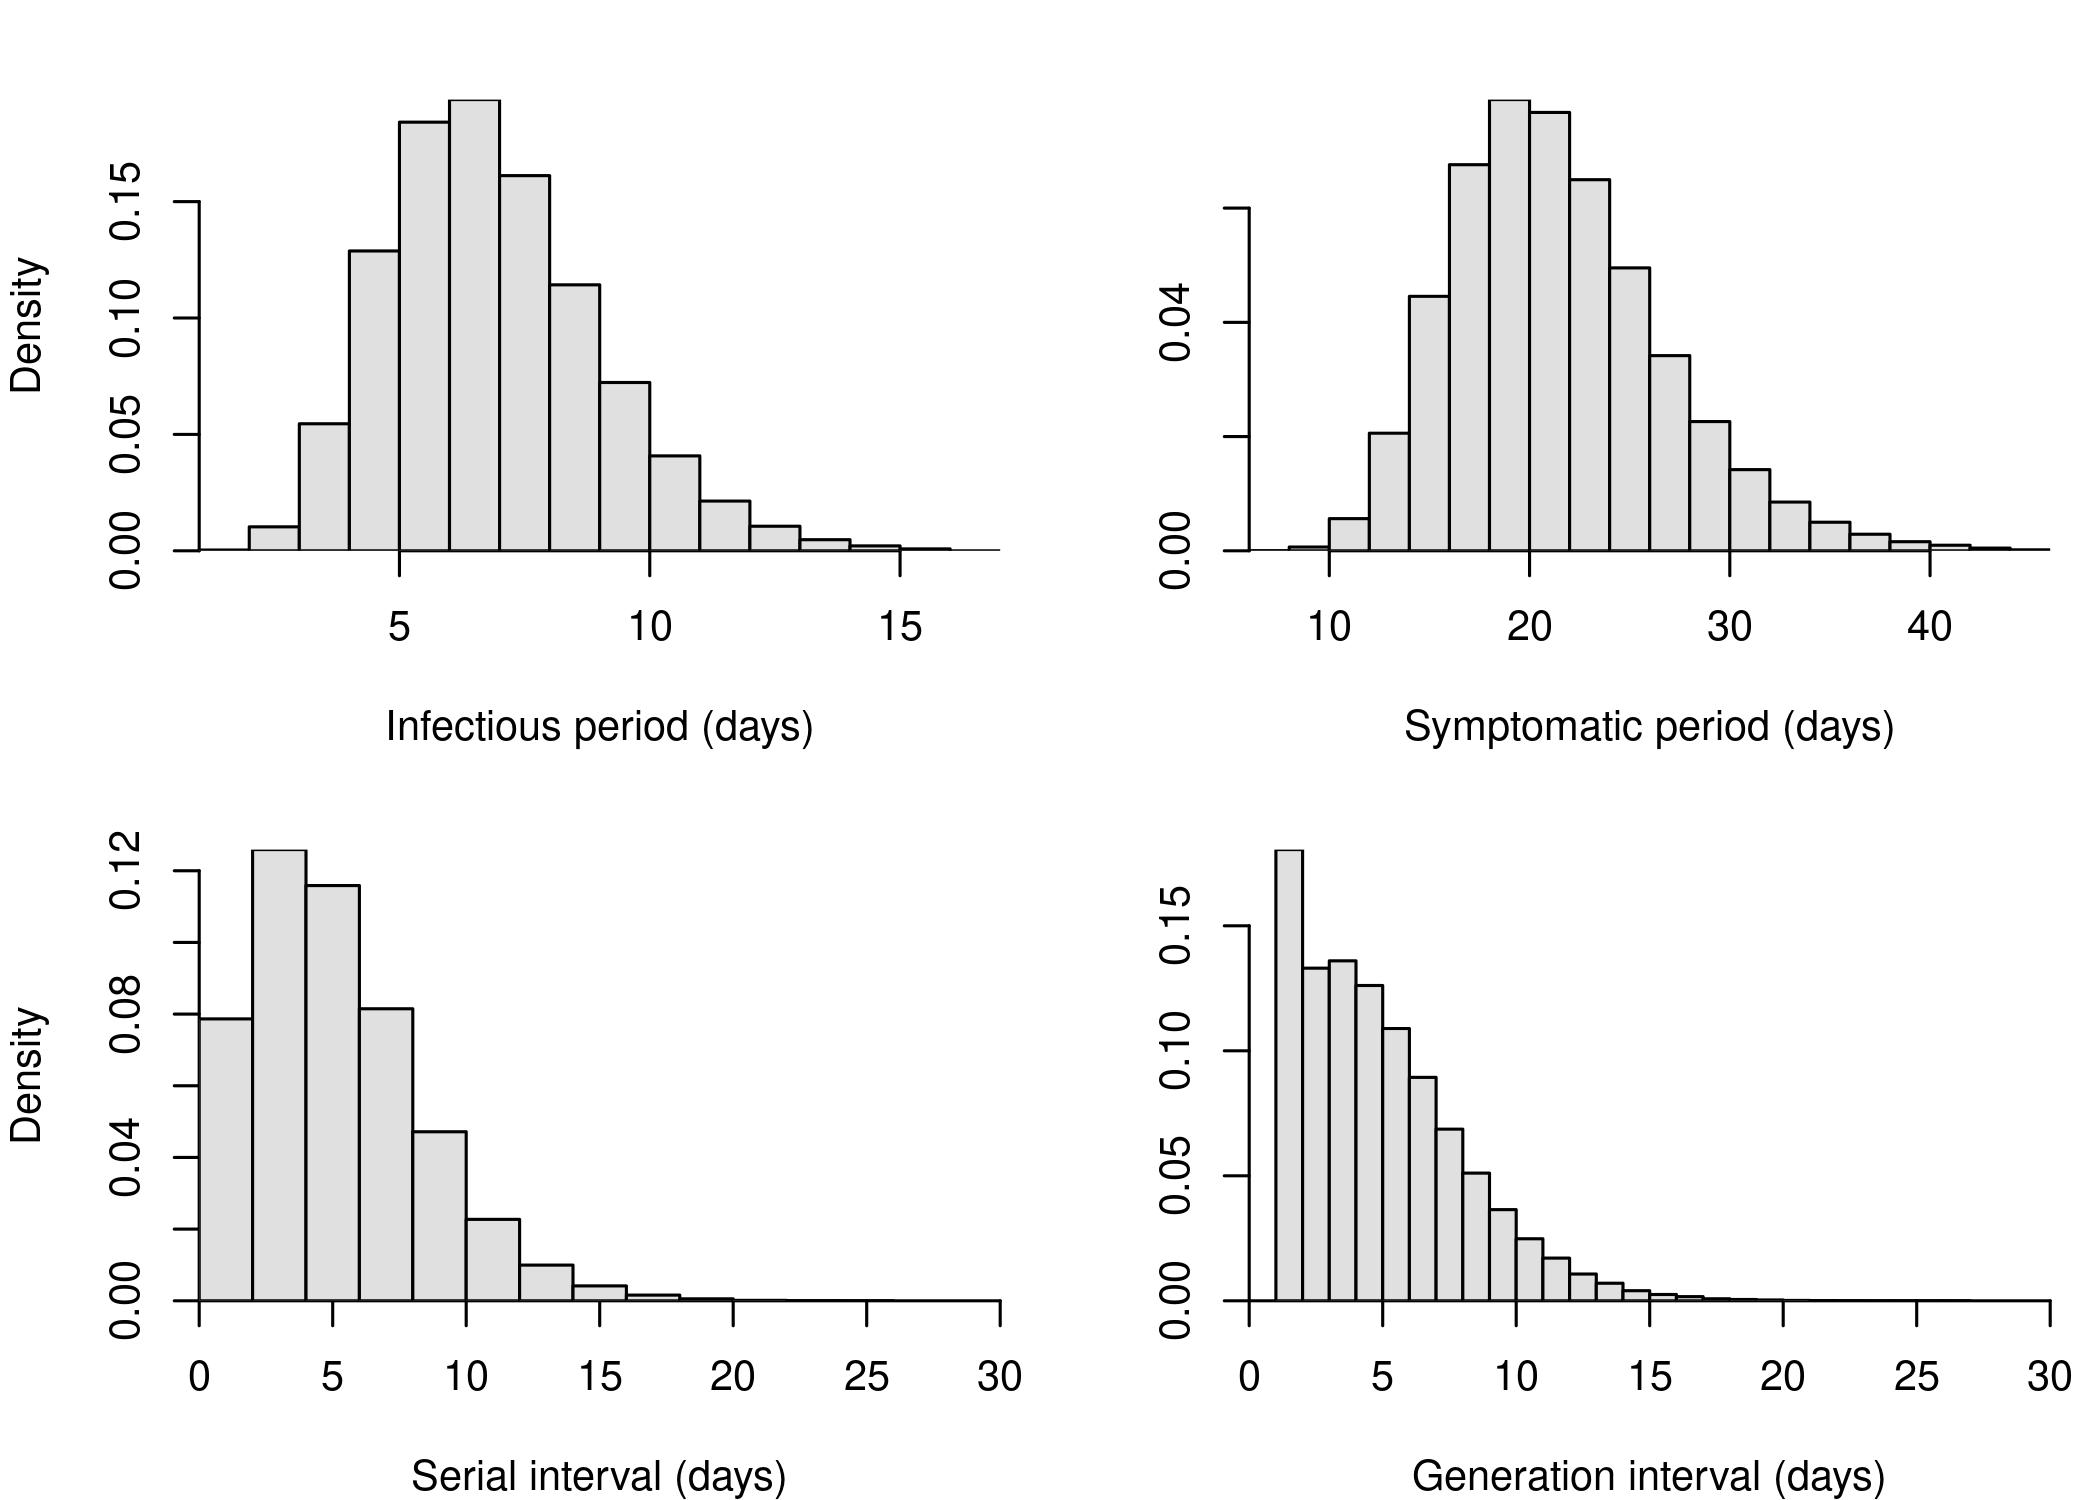
\includegraphics[width=\textwidth]{../figures/report_figure_parameter_periods.jpeg} 
\caption{\label{fig_params_periods}The distribution of the infectious period, symptomatic period, serial interval, and generation interval. The infectious period starts 2 days before the onset of symptoms.}
\end{figure}


\begin{figure}[hb!]
\centering
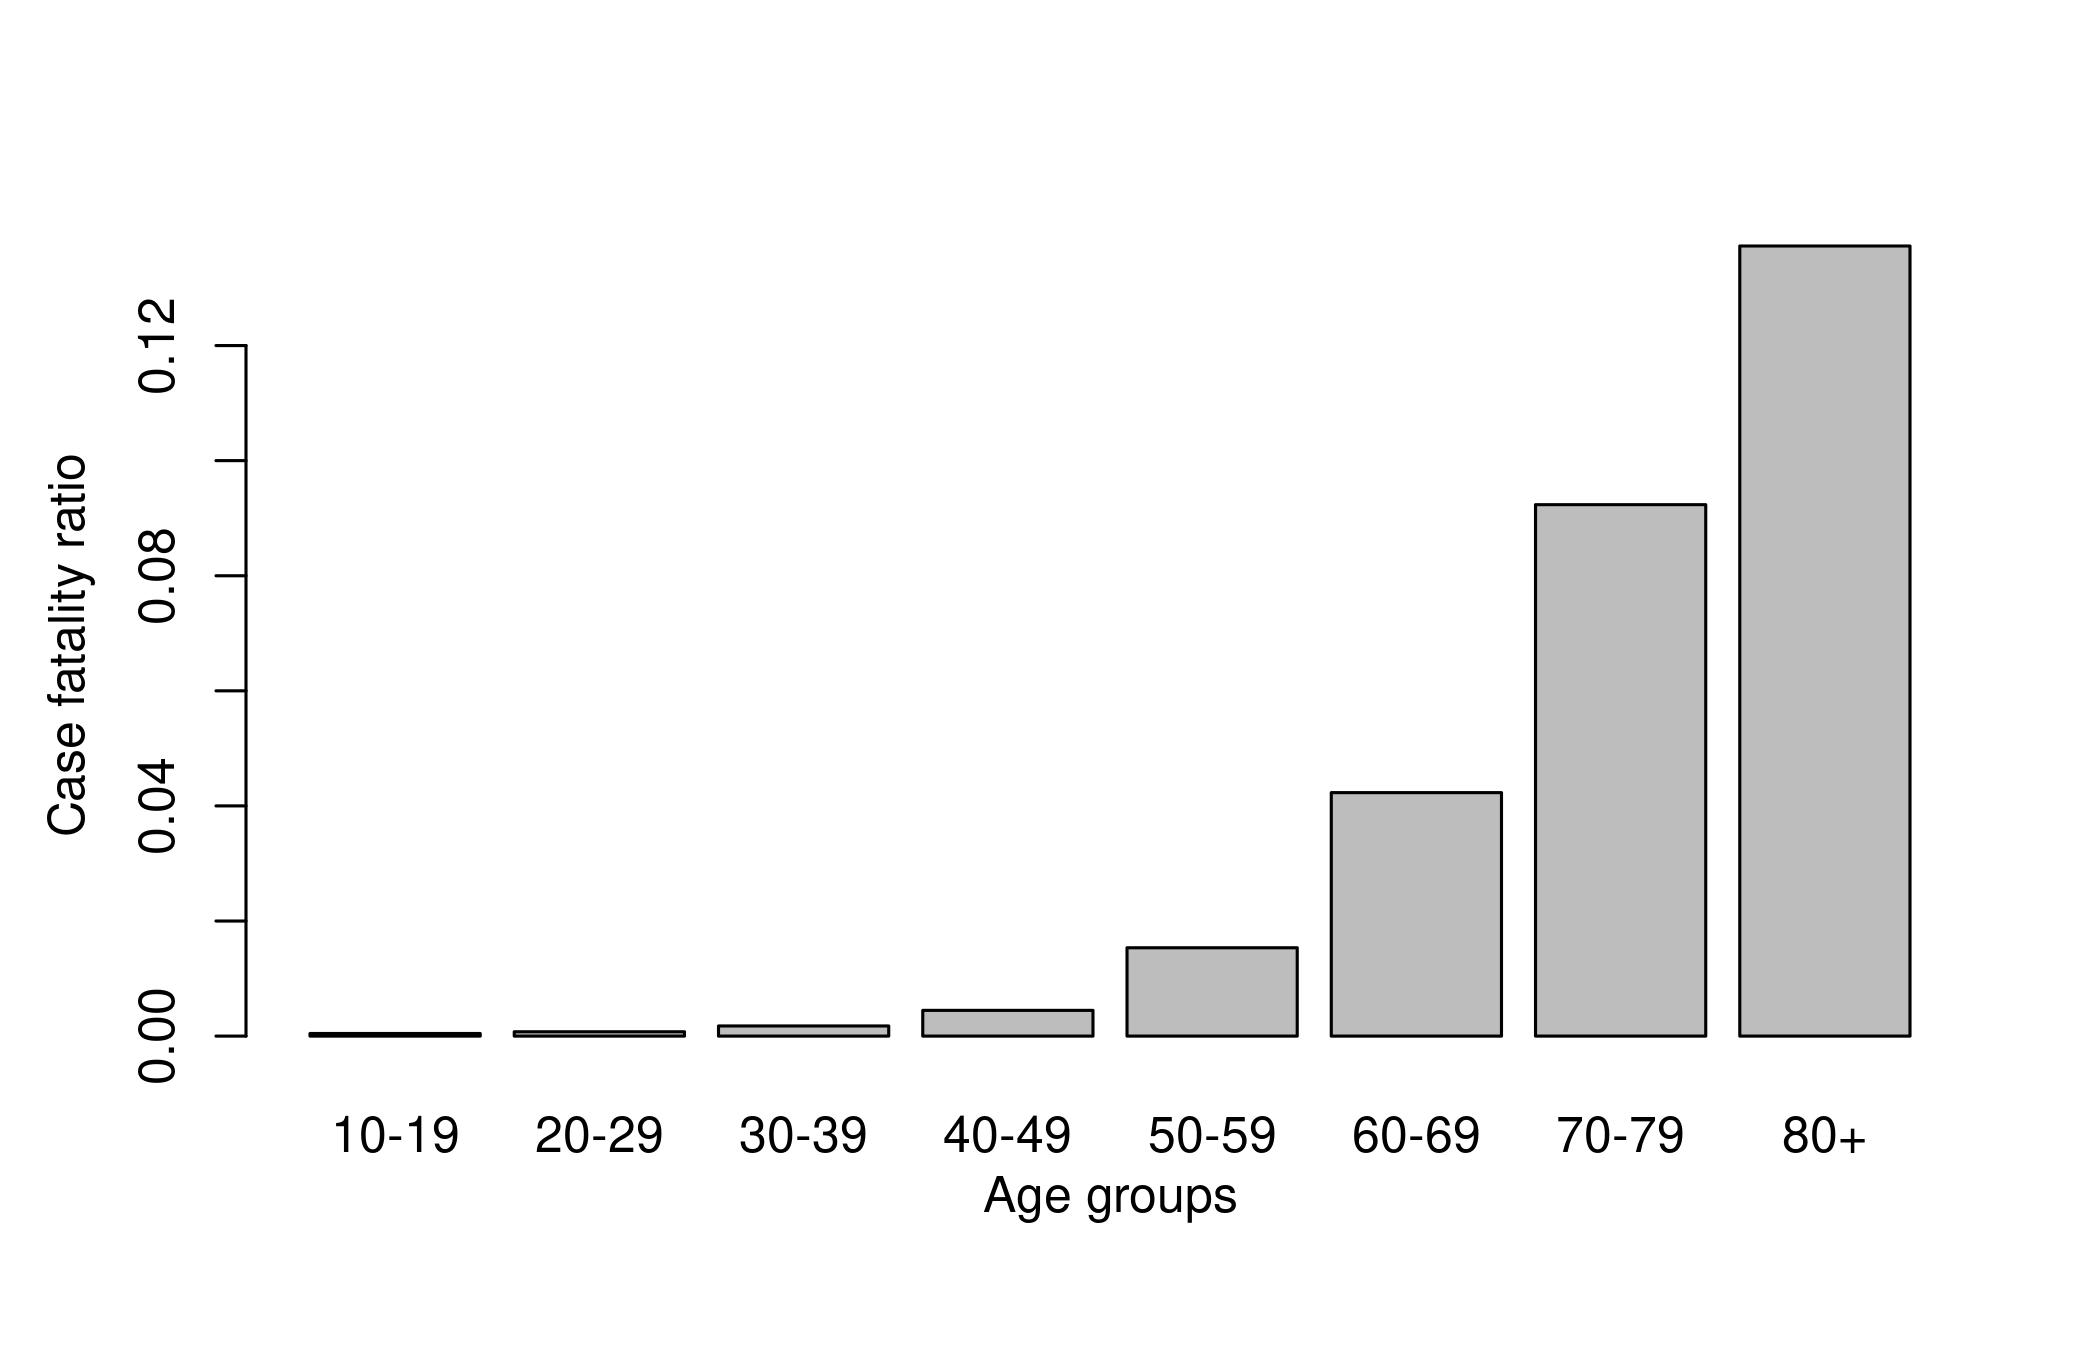
\includegraphics[width=\textwidth]{../figures/report_figure_age_CFR.jpeg} 
\caption{\label{fig_age_cfr} The age distribution in the case fatality risk, taken from Wu et al.}
\end{figure}

\begin{figure}[hb!]
\centering
\includegraphics[width=\textwidth]{../figures/report_figure_age_symptoms.jpeg} 
\caption{\label{fig_age_symp} The age distribution in the probability that a case shows symptoms.}
\end{figure}



\end{document}
%%% Local Variables:
%%% mode: latex
%%% TeX-master: t
%%% End:
